\begin{frame}{ЭПР-парадокс}
 \begin{columns}
   \column{0.4\textwidth}
   \begin{figure}
     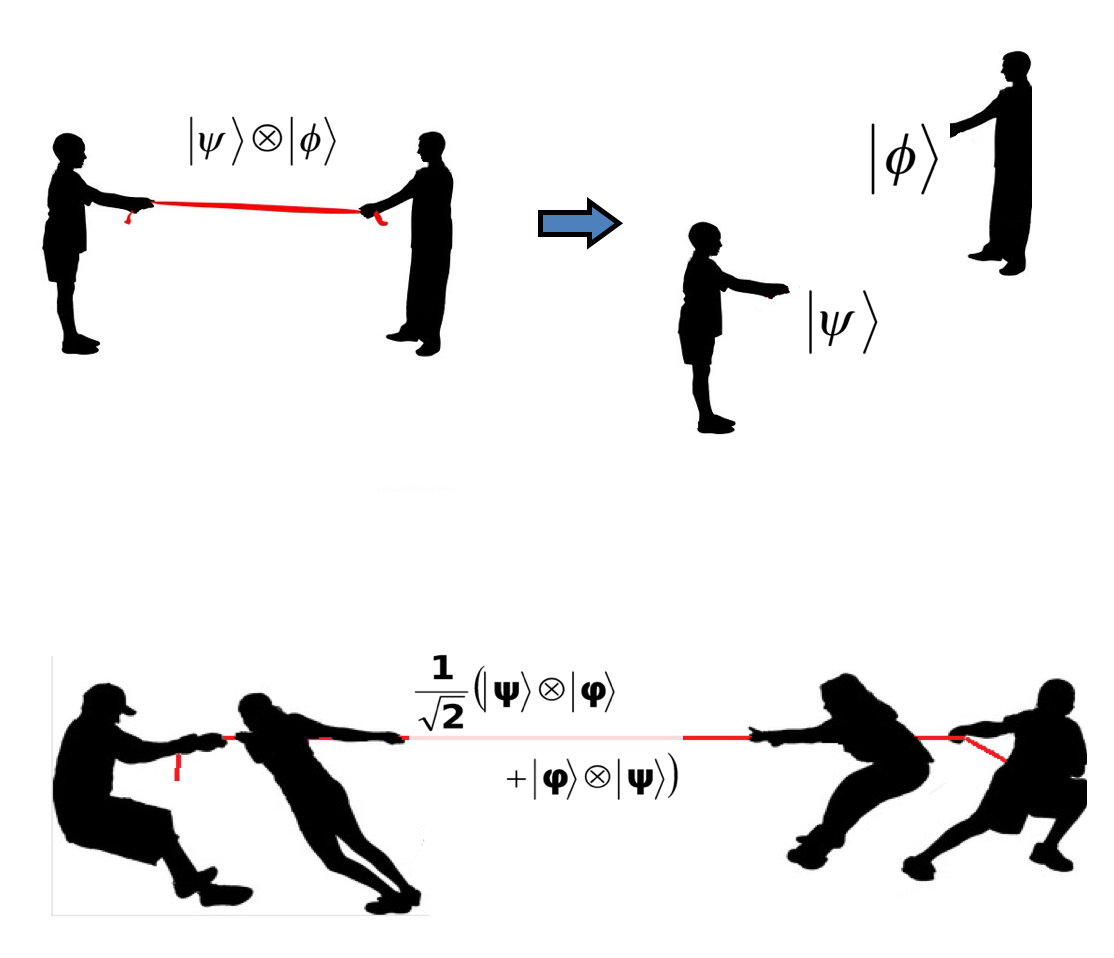
\includegraphics[width=\textwidth]{bi-entanglement.png}
   \end{figure}

   \column{0.5\textwidth}
   \begin{block}{}
     Работа Эйнштейна—Подольского-Розена\footnote[frame]{A. Einstein, B. Podolsky, and N. Rosen \textit{Phys. Rev.} \textbf{47}, 777 (1935)}
     указывала на неполноту квантовой механики с помощью мысленного эксперимента,
     заключающегося в измерении параметров микрообъекта косвенным образом,
     без непосредственного воздействия на этот объект.
   \end{block}
   \begin{block}{}
      В 2008 году был проведен эксперимент\footnote[frame]{T. Scheidl et al. \textit{PNAS} \textbf{107}, 46, 19708-19713 (2010)},
      который подтвердил нелокальный\footnote[frame]{J.S. Bell \textit{Physics Physique Fizika} \textbf{1}, 195 (1964)}
      характер квантовой теории.
   \end{block}
 \end{columns}
\end{frame}
\note{
  Первой работой в контекте квантовых корреляций принято считать статью опубликованную группой авторов ЭПР в 35 году.
  В работе обсуждалось парадоксальное поведение квантовой теории.
  Было показано, что существуют такие состояния,
  которые остаются взаимосвязанными даже за пределами светового конуса.

  Таким образом возможно измерение параметров удаленных микрообъектов косвенным образом.

  Разумеется вокруг работы разгорелись споры.

  В 64 году Джон Стюарт Белл предложил эксперимент, результат
  которого однозначно определял возможность таких корреляций.

  В 70 году Джоном Клаузером и  Аленом Аспе независимо были проведены первые эксперименты,
  которые подтвердили нелокальный характер квантовой теории.

  В настоящее время признано, что запутанность является ключевой концепцией квантовой теории.

  % Первый эксперимент был проведен Джоном Клаузером в 1972 (википедия).
  % Второй первый эксперимент был проведен Аленом Аспе в 70е.
  % (Alain Aspect Phys. Rev. D 14, 1944 – Published 15 October 1976)
  % И затем было еще много экспериментов.

  % В 2010 году Джон Клаузер, Ален Аспе и Антон Цайлингер стали лауреатами премии Вольфа по физике «за фундаментальный концептуальный и экспериментальный вклад в основы квантовой физики, в частности за серию возрастающих по сложности проверок неравенств Белла (или расширенных версий этих неравенств) с использованием запутанных квантовых состояний»
}

\begin{frame}{Бинарная запутанность}
  \begin{columns}
    \column{0.57\textwidth}
    $$
      \left| \Psi \right\rangle
      = \frac{
        \left| \uparrow\uparrow \right\rangle +
        \left| \downarrow\downarrow \right\rangle
      }{\sqrt{2}}
    $$
    \begin{block}{Критерии запутанности}
      \begin{itemize}
        \item Энтропия фон-Неймана \\
          {\footnotesize C.H.Bennett et al. \textit{Phys. Rev. A} \textbf{54}, 3824 (1996)}
        \item Критерий Вуттерса \\
          {\footnotesize W.K. Wootters, \textit{Phys. Rev. Lett.} \textbf{80}, 2245 (1998)}
        \item Мера Шмидта \\
          {\footnotesize Eisert J. and Briegel H. J. \textit{Phys. Rev. A} \textbf{64}, 022306 (2001)}
        \item ...
      \end{itemize}
    \end{block}

    %\begin{example}
    %  Запутанность в нитрозильном комплексе железа (НКЖ)\footnote[frame]{S. M. Aldoshin, E. B. Feldman, and M. A. Yurishchev, \textit{JETP} \textbf{107}, 5, 804–811 (2008)}.
    %\end{example}

    \column{0.4\textwidth}
    %\vspace{-2mm}
    \begin{figure}
      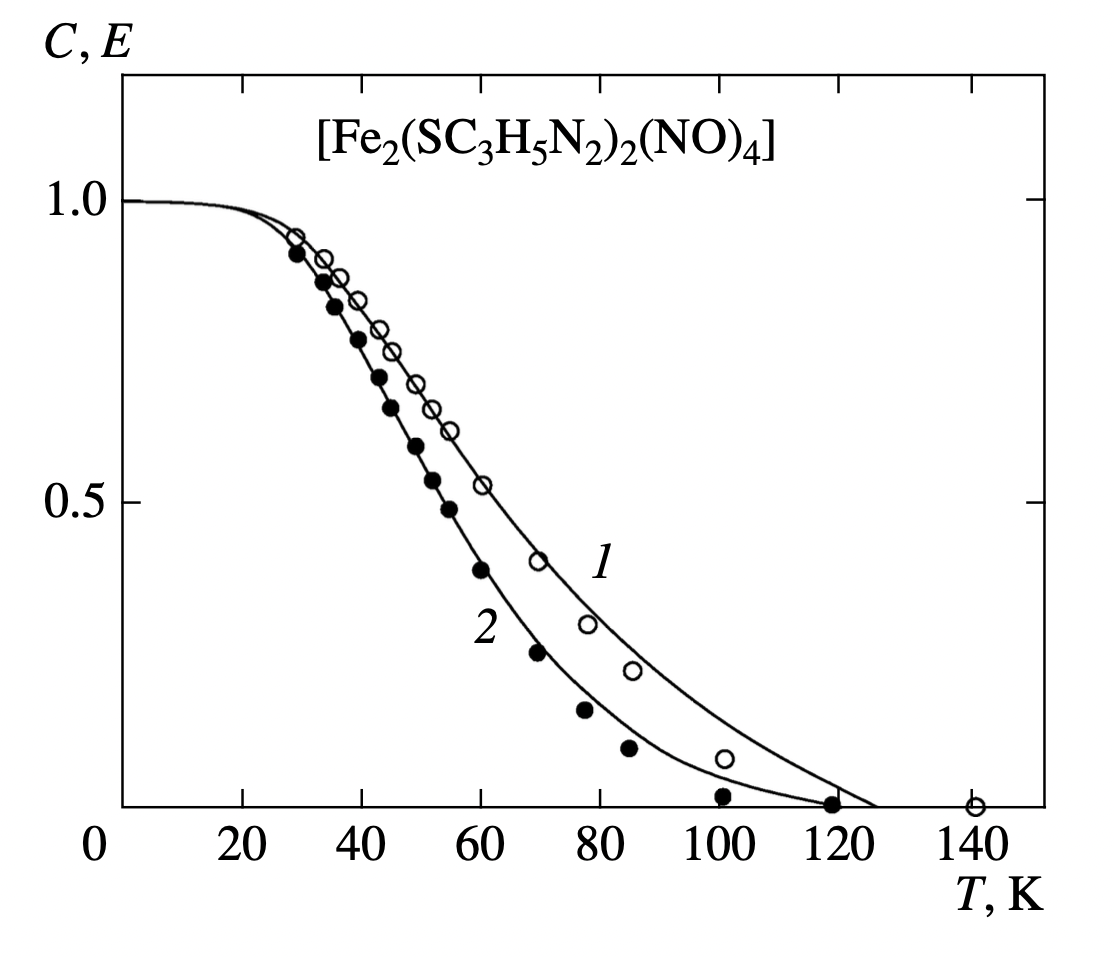
\includegraphics[width=\textwidth]{bi-entanglement-jetp2008.png}
      \captionsetup{skip=-2mm}
      \caption{Температурная зависимость согласованности (1) и запутанности (2) для нитрозильного комплекса железа\footnote[frame]{S. M. Aldoshin, E. B. Feldman, and M. A. Yurishchev, \textit{JETP} \textbf{107}, 5, 804–811 (2008)}.}
    \end{figure}
  \end{columns}
\end{frame}
\note{
  Определения таких состояний нетривиальная задача.
  В действительности, чтобы показать, что состояние запутанно нужно еще угадать с проективными измерениями,
  так как в произвольном базисе нельзя установить факт наличия запутанности.

  Эта задача уже хорошо разработана
  и было предложено множество критериев для выявления таких корреляций.
  например  мера Шмидта, согласованность Вуттерса, энропия фон-Неймана.


  Этот эффект хорошо изучен экспериментально, в качестве примера
  на слайде приведен результат из работы нашего института.
  Это температурная зависимость величины запутанности
  подсчитаной на основе согласованности в нитрозильном комплексе железа.
  Линии это теоретический расчет, точки это эксперимент.

  Такие результаты удается получит благодаря тому, ё
  что согласованность Вуттерса удалось связать с магнитной восприимчивостью атиферомагнитного димера.
}

\begin{frame}{Квантовые технологии}
  \begin{columns}
   \column{0.6\textwidth}
   \begin{figure}
     \begin{subfigure}[t]{0.33\textwidth}
       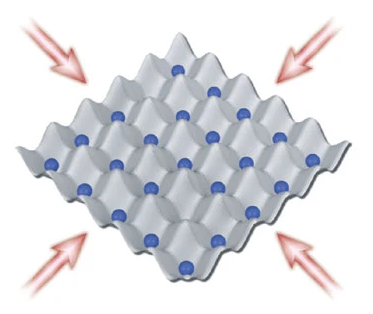
\includegraphics[width=\textwidth]{ultracold-atoms.png}
       %\captionsetup{labelformat=empty}
       \caption{Ultracold atoms}
       \label{fig:ultracold-atoms}
     \end{subfigure}
     \begin{subfigure}[t]{0.33\textwidth}
       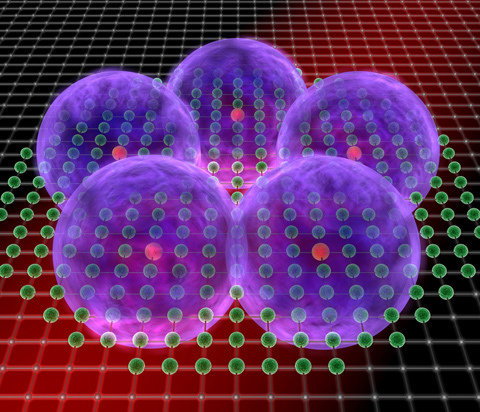
\includegraphics[width=\textwidth]{ridberg-atoms.png}
       %\captionsetup{labelformat=empty}
       \caption{Rydberg atoms}
     \end{subfigure}
     % \vspace*{2mm}
     \vfill
     \begin{subfigure}[t]{0.33\textwidth}
       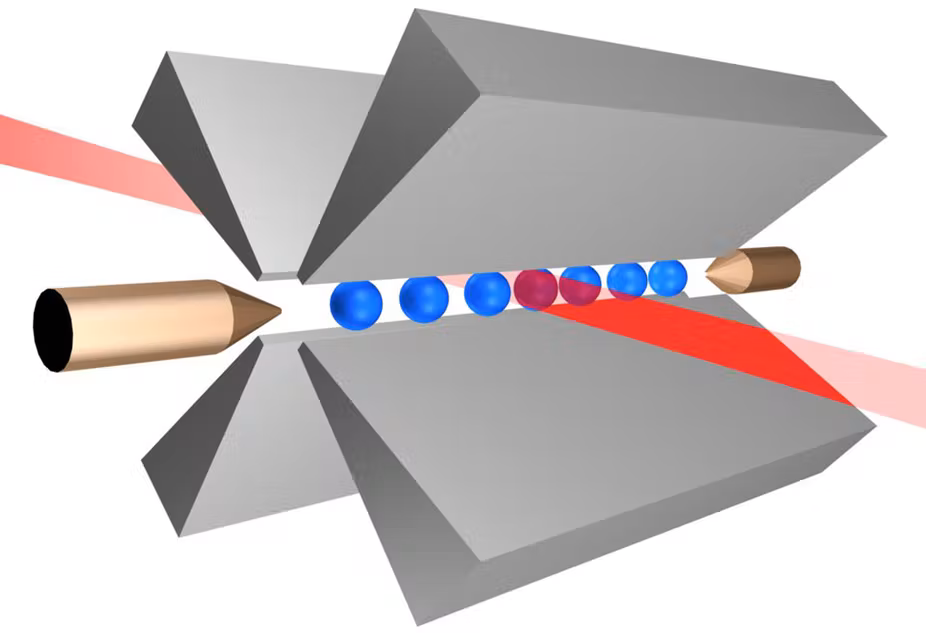
\includegraphics[width=\textwidth]{trapped-ions.png}
       %\captionsetup{labelformat=empty}
       \caption{Trapped ions}
     \end{subfigure}
     \begin{subfigure}[t]{0.33\textwidth}
       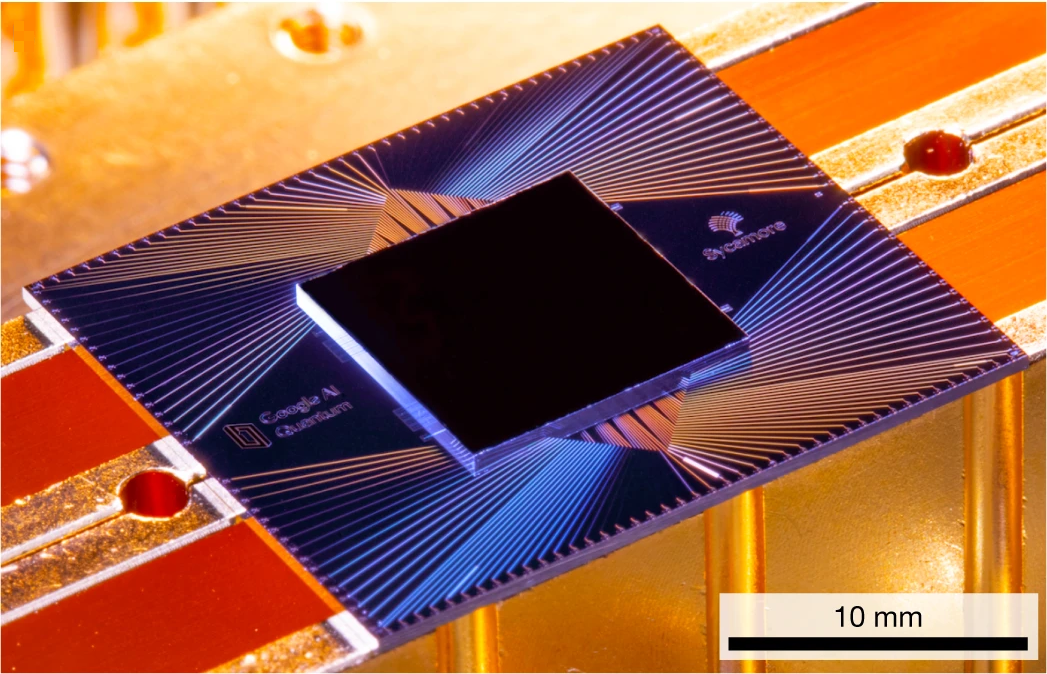
\includegraphics[width=\textwidth]{sycamore.png}
       %\captionsetup{labelformat=empty}
       \caption{SC qubits}
     \end{subfigure}
     \caption{
       Квантовые платформы.
       % (\ref{fig:ultracold-atoms})~{Bloch, I. Nature 453, 1016–1022 (2008)}
     }
   \end{figure}

   \column{0.4\textwidth}
   \begin{figure}
       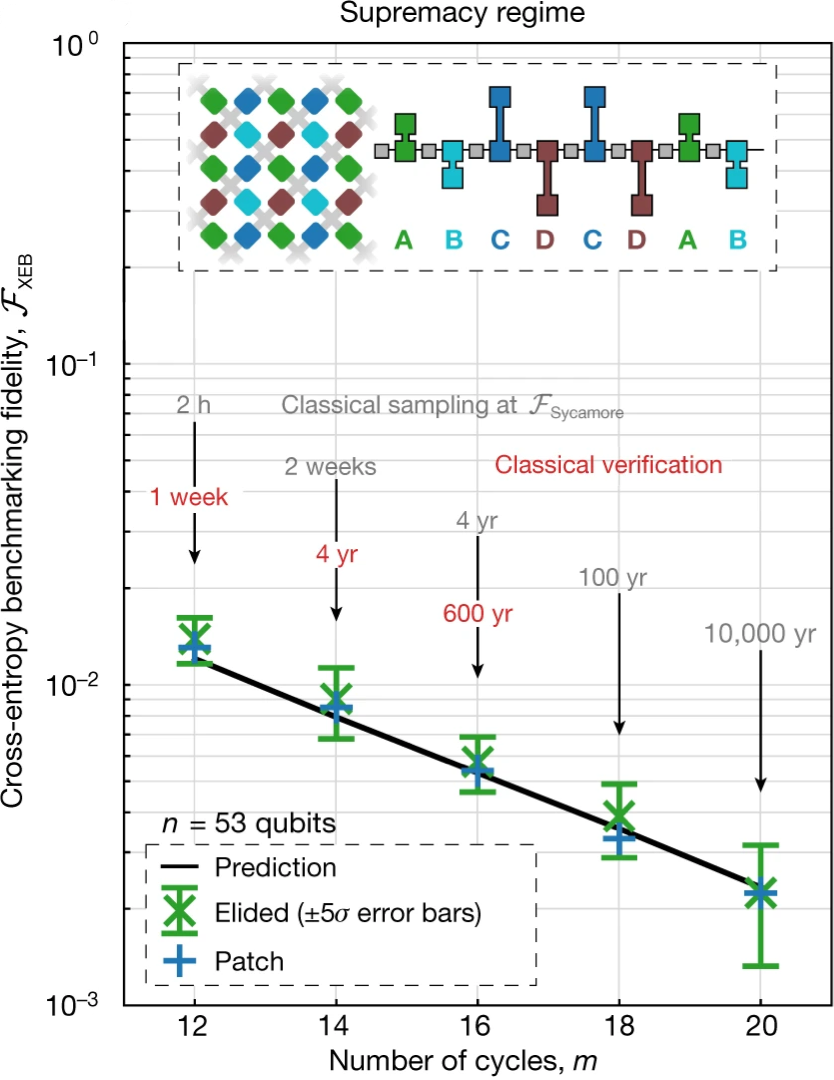
\includegraphics[width=0.8\textwidth]{sycamore-supemancy.png}
       % \captionsetup{labelformat=empty}
       \caption{
         % F. Arute et al., Nature 574, 505 (2019)
         Nature 574, 505 (2019)
       }
     \end{figure}
   \end{columns}
\end{frame}
\note{
  Тем неменее когда мы говорим о квантовом превосходстве
  мы иммеем ввиду большое количество взаимодействующих кубитов.
  Сейчас это порядка 50.
  Это значит, что главным реусурсом является не бинарная запутанность, а многокубитная.
  Предпринятые в данной работе попытки количественного определения запутанности мотивированы желанием понять и количественно оценить эти ресурсы.


  % \textbf{ЯМР}
  % ЯМР был первым, но он негодится для вычислений (нет чистых состояний).
  % Отлично подходит для исследований.
  % Много наработок.
%
  % Исследуется все гильбертого пространство.
  % Квантовое превосходство  на программируемом сверхпроводящем процессоре.
  % Запутанные состояния являются важным ресурсом в квантовых вычисления:
  % Например, недавно продемонстрированное группой Мартинеса квантовое превосходство [1] на программируемом сверхпроводящем процессоре связано с понятием запутанноси
}


\begin{frame}{Цели и задачи}
  \textbf{Целью данной работы} является теоретическое исследование многочастичной запутанности в системах с большим количеством частиц $(>200)$ в рамках МК спектроскопии ЯМР,
а также развитие методов экспериментального измерения величин квантовой информации Фишера и косой информации Вигнера-Янасе.
\end{frame}
\note{
  Целью данной работы является теоретическое исследование многочастичной запутанности в системах с большим количеством частиц.
  Так как мы хотим исследовать действительно большие системы,
  то наиболее удобным вариантом является твердотельный ЯМР.

  Как будет показано ниже, определение количества запуттаных спинов,
  это частный случай более сложной фундаментальной проблемы,
  а конкретно измерения квантовых информационных величин.
  Поэтому более общая цель работы это развитие экспериментальных методов измерения квантовой информации Фишера и косой информации.
}

\begin{frame}{Положения, выносимые на защиту}
  \begin{enumerate}
  \item 
  Разработана теория МК ЯМР для системы эквивалентных спинов при произвольной температуре.
  
  \item 
  Исследована температурная зависимость многочастичной запутанности в нанопоре, 
  когда система приготовлена в термодинамическом равновесном зеемановском и дипольно упорядоченном состояниях.
  
  \item
  Исследована многочастичная запутанность в квазиодномерных цепочках ядерных спинов в зависимости от параметров цепи и температуры.
  
  \item 
  Предложен метод экспериментального измерения точного значения косой информации Вигнера-Янасе в рамках МК спектроскопии ЯМР.
  
  \item 
  Проведено сравнение оценок многочастичной запутанности, полученных на основе квантовой информации Фишера и косой информации Вигнера-Янасе.
\end{enumerate}
\end{frame}
\note{
    Проведенные исследования позволяют заключить,
    что МК-спектроскопия ЯМР является тонким и полезным методом для исследования различных проблем квантовой информатики.
    В частности, это очень эффективный метод исследования квантовой запутанности.
}

\begin{frame}{Научная новизна и практическая ценность}
  \begin{block}{Научная новизна.}
    В данной работе была разработана теория МК ЯМР для нанопоры при произвольной температуре,
что позволило впервые теоретически исследовать температурную зависимость многочастичной запутанности в системе из более чем 200 взаимодействующих частиц.
Также в данной работе был разработан метод определения величины косой информации Вигнера-Янасе в МК эксперименте ЯМР.
  \end{block}

  \begin{block}{Практическая ценность.}
   Так как косая информация Вигнера-Янасе нашла много применений в квантовой теории информации, %~\cite{Wigner1963, Luo2017},
предлагаемый в данной работе метод определения ее величины
не только позволяет исследовать многочастичную запутанность методами МК ЯМР,
но и открывает возможность решения широкого класса задач в этой области.
  \end{block}
\end{frame}
